
\documentclass[%
 preprint,
%superscriptaddress,
%groupedaddress,
%unsortedaddress,
%runinaddress,
%frontmatterverbose, 
%preprint,
%showpacs,preprintnumbers,
%nofootinbib,
%nobibnotes,
%bibnotes,
 amsmath,amssymb,amsfonts,
 aps,
%pra,
%prb,
%rmp,
%prstab,
%prstper,
%floatfix,
]{revtex4-1}
\usepackage{txfonts}
\usepackage{graphicx} 
\usepackage{rotating}
\usepackage{changepage}
\usepackage{color}
\definecolor{light-gray}{gray}{0.95}

\usepackage{listings}
\lstset{
                breaklines=true,
                backgroundcolor=\color{light-gray},
                numbersep=5pt,
                xleftmargin=.5in,
                xrightmargin=.5in} 

%%%%%%%%%%%%%%%%%%%%%%%%%%%%%%%%%%%%%%%%%%%%%%%%

\begin{document}

\newcommand{\qq}{\symbol{34}} % 34 is the decimal ascii code for "


\title[TempoNest]{TempoNest - Installation and Usage }
\author{Lindley Lentati}
\email[]{ltl21@cam.ac.uk}
%\homepage[]{Your web page}
%\thanks{}
%\altaffiliation{}
\affiliation{Astrophysics Group, Cavendish Laboratory, JJ Thomson Avenue,  Cambridge, CB3 0HE, UK}

\maketitle

\label{firstpage}
\section{Introduction}

TempoNest provides a means of performing a simultaneous analysis of the either the linear, or non linear deterministic pulsar timing model and additional stochastic parameters.  It uses the Bayesian inference tool MultiNest \cite{2008MNRAS.384..449F, 2009MNRAS.398.1601F} to efficiently explore this joint parameter space, whilst using TEMPO2 (\cite{2006MNRAS.369..655H, 2006ChJAS...6b.169H, 2004MNRAS.353.1311H}). as an established means of evaluating the timing model at each point in that space.  The former can be downloaded at \footnote{http://ccpforge.cse.rl.ac.uk/gf/project/multinest/} and the latter is available at \footnote{http://sourceforge.net/projects/tempo2/}.  

This document is designed to serve as an installation and operating guide for TempoNest, specific details of, for example, the timing model fit by Tempo2, will not be included but are available in the references above.

Section \ref{Section:Install} provides details of the installation process,  Section \ref{Section:Model} describes the different models currently available, Sections \ref{Section:params} and \ref{Section:Advanced} describes all the user set parameters available in TempoNest.  In Section \ref{Section:Sim} we describe the simulation facilities present in TempoNest and in Section \ref{Section:Output} we describe the content of the output files produced by the Bayesian analysis.  Finally in Section \ref{Section:Example} a set of complete examples are given using the data that is included in the Examples sub-folder.

If you have any questions, or problems regarding the installation, or usage, please do not hesitate to contact me, and I will be happy to assist as much as possible.
 
\section{Installation}
\label{Section:Install}
Compilation has been tested using gcc 4.6.1.  Other compilers, or combinations of compilers are thus currently unsupported.

TempoNest has dependencies upon both Tempo2 and MultiNest, however in addition it requires access to gsl functions, and an installation of either the LAPACK linear algebra library or, if TempoNest is to be run using a GPU, the CULA linear algebra library.

\subsection{Install MultiNest}
Download the latest version of MultiNest (3.x) (Note: to use MultiNest you will need to have access to the lapack linear algebra library which can be downloaded from \footnote{http://www.netlib.org/lapack/})  and open the file Makefile in the root directory.    You will need to change the compilers so that:
%

\begin{lstlisting}
FC = gfortran
CC = gcc
CXX = g++
FFLAGS += -03 -ffree-line-length-none
CFLAGS += -03
LAPACKLIB = -llapack

\end{lstlisting}


%
then type make and allow the source code to compile.  You will then need to create a shared version of the libnest3.a library, which can be done with the command:
\begin{lstlisting}
make libnest3.so
\end{lstlisting}
 %
 The auto-configure script for TempoNest will then look for this file through the environment variable MULTINEST$\_$DIR

\subsection{Install Tempo2}

Download the latest version of Tempo2 available via cvs using the command:
\begin{lstlisting}
cvs -z3 -d:pserver:anonymous@tempo2.cvs.sourceforge.net:/cvsroot/tempo2 co -P tempo2
\end{lstlisting}


Enter the root directory, and copy the folder T2runtime to a location of your choice.  You will have to set the environment variable TEMPO2 to be the location of this directory.

Then type:
\begin{lstlisting}
./bootstrap
./configure --prefix = install directory
\end{lstlisting}
 %
 and allow the script to run, this will set up the Makefile for you without you having to do anything yourself.  Once the configure script has run type:
\begin{lstlisting}
make
make install
make plugins
make plugins-install
\end{lstlisting}

This will compile and install the code to the directory given by the prefix command.  The libraries and include files you will need to link to TempoNest will be installed to the lib and include subdirectories in the install folder, which should be stored as the environment variables TEMPO2$\_$LIB and TEMPO2$\_$INC respectively.

\subsection{Install TempoNest}

TempoNest supports both CPUs and GPUs, however at this stage the configure script only supports a CPU installation, with a GPU installation requiring more manual intervention.


\subsubsection{TempoNest without GPUs}

Enter the root folder containing TempoNest and type:
%
\begin{lstlisting}
./autogen.sh
./configure
\end{lstlisting}
%
This should produce the Makefile required to install TempoNest.  You should check the output of this to make sure that the multinest and tempo2 libraries were found correctly.
Then simply type:
\begin{lstlisting}
make && make install
\end{lstlisting}
%
and the TempoNest plug-in will be compiled and copied to your Tempo2 plug-in directory.

\subsubsection{TempoNest with GPUs}

In the autoconf subdirectory of the TempoNest source folder there is a file cula.m4, you will first have to open this and remove the word "Fake" from lines 66 and 70, which will cause the configure script to correctly identify the CULA libraries and use the correct compilation options when producing the plug-in.

You will then need to compile the file TempoNestGPUFuncs.cu with the nvcc compiler  before you run the configure scripts to form a shared object libTNGPU.so that can then be linked against the TempoNest install.  This can be done with the following:

\begin{lstlisting}
nvcc -arch sm_20 -Xcompiler -O3 --shared -I${CULA_INC_PATH} -o libTNGPU.so TempoNestGPUFuncs.cu -L${CULA_LIB_PATH_64} -lcula_lapack -lcuda --compiler-options '-fPIC' 
\end{lstlisting}
%


Move the file libTNGPU.so to the directory TEMPO2$\_$LIB and then as with the normal install type:
\begin{lstlisting}
./autogen.sh
./configure
make && make install
\end{lstlisting}
%
This should detect the CULA libraries, and the GPU functions and allow you to use a GPU for all linear algebra in TempoNest.


\section{Interface and Operation}
\label{Section:Interface}

TempoNest is designed to be simple to use for anyone with (or indeed, without) previous experience with Tempo2.  As such, once any relevant parameters have been set, given a par file X.par, and a tim file X.tim, TempoNest can be run from the command line in it's root directory using the command:
%
\begin{lstlisting}
./tempo2 -gr temponest -f X.par X.tim
\end{lstlisting}
%
The parameters that have been set to fit in the .par file will be those that are included in the timing model fit in TempoNest, therefore anyone used to using Tempo2 can immediately analyse their data using TempoNest.  In the following sections we will describe in more detail the different settings available for the analysis of pulsar timing data, as well as how to simulate data in TempoNest itself.


\section{Included Models}
\label{Section:Model}

TempoNest allows for the simultaneous Bayesian  analysis of both the deterministic timing model, and additional stochastic signals beyond the white noise described by the TOA error bars that may be present in the data.  For a general overview of Bayesian analysis and the sampler MultiNest, a detailed description of all available model choices present in TempoNest, and examples of its application to simulated data refer to the TempoNest paper (in prep).  Below we will summarise the key aspects of the included models, without going into the mathematical details.

\subsection{The Timing Model}
\label{section:timingmodel}
TempoNest uses Tempo2  to evaluate the deterministic pulsar timing model for those parameters in the pulsar par file.
One consideration here arises from the fact that Tempo2 necessarily uses long double precision to store the timing model parameters, however MultiNest operates at double precision.  MultiNest therefore parameterises the timing model fit for each parameter $m$ in terms of deviations from some reference value $m_0$ in multiples of a scaling parameter $m_{\epsilon}$.   Therefore, in every likelihood evaluation MultiNest will select a value $m_p$ for each timing model paratmer $m$ which is then transformed to $m_t$ by:
%
\begin{lstlisting}[mathescape]
$m_t = m_0 \pm (m_p \times m_{\epsilon} ) $
\end{lstlisting}
%
which can then be passed to Tempo2 in order to evaluate the timing model for the set of timing model parameters $m_t$.


\subsection{Additional White Noise}
\label{Section:White}


When dealing with pulsar timing data, the properties of the white noise can be separated into two components:

\begin{description}
  \item[1] For a given pulsar, each TOA has an associated error bar, the size of which will vary across a set of observations.  We can therefore introduce an extra free parameter, an EFAC value, to account for possible mis-calibration of this radiometer noise \cite{2006MNRAS.369..655H}.  The EFAC parameter therefore acts as a multiplier for all the TOA error bars for a given pulsar, observed with a particular system. TempoNest allows for either a single EFAC parameter to be estimated for all TOAs for a given pulsar, or, where the observing system has been flagged for each TOA, a separate EFAC can be included for each system.\\
 \item[2] A second white noise component, independent of the size of the error bars is also used to represent some additional source of time independent noise.  We call this parameter EQUAD.  In principal this parameter represents something physical about the pulsar, such as an intrinsic jitter in the pulse emission time and so should be independent of the observing system.  As such a single EQUAD parameter is available to include for all TOAs.
\end{description} 
%
We can therefore rewrite the error $\sigma_i$ associated with each TOA $i$ as $\hat{\sigma}_i$ so that:
\begin{equation}
\hat{\sigma}_i^2 = (\alpha_i\sigma_i)^2 + \beta^2
\end{equation}
%
where $\alpha$ and $\beta$ represent the EFAC and EQUAD parameters applied to TOA $i$ respectively.  


\subsection{Red Noise and DM Models}

TempoNest currently supports two methods of modelling either the red noise or DM.  The time domain methods described in (\cite{2012arXiv1202.5932V} henceforth vHL2013) and Lee et al 2013 (in prep) where a power law is used to model either the red noise or DM, and the model-independant frequency domain method described in (Lentati L. et al. 2013 henceforth L2013) where the power at each frequency included in the model is parameterised separately.  TempoNest also allows for a power law to be fit to the same set of frequencies that are used in the model independant method so that both modelled and model independant methods can be used simultaneously.


\section{TempoNest Parameters}
\label{Section:params}

In the folder Examples/Example1 of the TempoNest source folder there is a file called defaultparameters.conf which contains all the user defined parameters necessary to run TempoNest.  In this section we will provide a complete list of all these parameters and their function in the program.  Values listed here will be those set by default.

\subsection{General Parameters}

%
\begin{lstlisting}
root = results/Example1-
\end{lstlisting}
%
The root name for the output files generated by TempoNest, details of which will be described in Section \ref{Section:Example}.  In the Worked example this will result in a set of files being produced in the Example/results folder, each of which will have the prefix `Example1-' followed by the name of the pulsar, and the file extension.



\begin{lstlisting}
numTempo2its = 1;
\end{lstlisting}
%
The number of iterations to have Tempo2 perform before starting the analysis.  TempoNest takes the pre-fit values from this fit as the center of the prior for the following analysis, and the 1 sigma errors, redivded by the square root of the reduced chi square of the fit as the "sigma" value (see FitSig below).  Therefore if you wish to use the values in the .par file as the center of your prior this should be set to 1. However its value will depend critically on whether or not Tempo2 is able to converge on the problem you wish to analyse with TempoNest.  If convergence is not possible this should be set to 1, or 0 and the priors should be set manually as described in section \ref{Section:customPriors}.

\begin{lstlisting}
doLinearFit=0;
\end{lstlisting}
%
Toggles between performing the non linear analysis of the timing model (doLinearFit=0) and using the linear approximation evaluated at some point in the timing model parameter space  (doLinearFit=1) .  The point at which the linearisation occurs follows a hierarchal order depending on the options set in TempoNest.  If the central value for the prior on any of the timing model parameters has been set manually then these values will be used for the linearisation over all others.  If a maximum likelihood analysis has been performed over the joint parameter space, then the values for the parameters returned by this process will be used, otherwise if neither of these options have been taken, the parameter estimates made during the initial Tempo2 evaluation will be used.

\begin{lstlisting}
doMax=0;
\end{lstlisting}
%
Toggles between either performing a maximum likelihood analysis of the parameter space to be investigated (doMax=1) or not (doMax=0).  The values of the timing model parameters returned by this process supersedes those returned by the initial Tempo2 analysis, but are overwritten by any prior that has been set manually. 

\subsection{Marginalisation}

TempoNest allows you to marginalise analytically over subsets of timing model parameters in order to reduce the dimensionality of the problem.  For example, when fitting jumps the basis functions that describe the jump are linear, and so marginalising over the amplitudes can greatly simplify an analysis.  TempoNest supports several options for this process:

\begin{lstlisting}
doTimeMargin=0
doTimeMargin=1
doTimeMargin=2
\end{lstlisting}
%
These settings allow you to toggle between no marginalisation, marginalising over the quadratic spin down, and marginalising over all timing model models, except the jumps (0,1,2 respectively).

\begin{lstlisting}
doJumpMargin=0
doJumpMargin=1
\end{lstlisting}
%
These settings allow you to toggle between not marginalising over any jumps in the parameter file or marginalising over all of them (0,1 respectively).

Note that, if any analytical marginalisation is performed the offset is also marginalised over be default in the Tempo2 design matrix.

It is also possible to marginalise over customised sets of parameters.  This is done by setting a flag in the TempoPriors array corresponding to the particular parameter, for example, if the parameters to be fit were (RA, DEC, F0, F1, DM, PMRA, PMDEC, PX) and you wanted to marginalise over only DM analytically, you could include the following in the defaultparameters.conf file:

\begin{lstlisting}
TempoPriors[5][2]=1;
\end{lstlisting}
%
Here the 5 references the fact that it is the 5th parameter that Tempo2 will read in, and the 2 is the element where this information is kept.  For more information on setting custom priors see section \ref{Section:customPriors}.

\subsection{Model Selection}

\subsubsection{EFAC}

\begin{lstlisting}
incEFAC = 0;
\end{lstlisting}

Flag to include additional EFAC white noise parameters in the analysis.  Supports three possible values:

\begin{lstlisting}
0 : Include No Additional EFAC parameters 
1 : Include one EFAC parameter for all error bars
2 : Include one EFAC parameter for each -sys flag in  the tim file for all error bars associated with that flag
\end{lstlisting}


\subsubsection{EQUAD}

\begin{lstlisting}
incEQUAD = 0;
\end{lstlisting}

Flag to include an additional EQUAD white noise parameter in the analysis.  Supports two possible values:

\begin{lstlisting}
0 : Include No Additional EQUAD parameters 
1 : Include one EQUAD parameter for all TOA error bars
\end{lstlisting}

\subsubsection{Red Noise}

\begin{lstlisting}
incRED = 0;
\end{lstlisting}

Flag to include an additional red noise parameter in the analysis.  Supports three possible values:

\begin{lstlisting}
0 : Include No Additional Red Noise parameters 
1 : Include Red Noise using method vHL2013
2 : Include Red Noise using method L2013
3 : Fit a power law to the freqeuencies used in model 2 rather than allowing the power to vary independently
\end{lstlisting}

\subsubsection{DM}

\begin{lstlisting}
incDM = 0;
\end{lstlisting}

Flag to include an additional DM parameter in the analysis.  Supports three possible values:

\begin{lstlisting}
0 : Include No Additional DM parameters 
1 : Include DM using method Lee et al 2013
2 : Include DM using method Lentati et al 2013
3 : Fit a power law to the frequencies used in model 2 rather than allowing the power to vary independently
\end{lstlisting}

\begin{lstlisting}
numCoeff=3;
\end{lstlisting}
%
If incRED or incDM is set to 2 such that the red noise/DM model to be used is that of L2013, the numCoeff parameter sets the number of frequencies that should be included in the model.  If the observations span a length of time T, then the frequencies included will be n/T where n goes from 1 to numCoeff.

\subsection{Priors}

\begin{lstlisting}
customPriors = 0;
\end{lstlisting}

Priors in TempoNest can be handled in a variety of different ways, corresponding to different levels of control.  The simplest approach requires only a single prior to be set for each "class" of parameter, i.e. one prior is used for all timing model parameters, one prior is used for all EFACs etc.  This is achieved by setting customPriors =0.   However, if desired all the priors can be set manually using the setTNPriors function located in the TempoNestParams.c file which is accessed when customPriors = 1.  Below we will explain both the different approaches.

\subsubsection{Simple Priors (customPriors == 0)}

\begin{lstlisting}
FitSig = 4;
\end{lstlisting}

If customPriors is set to zero, then TempoNest will use the initial Tempo2 evaluation of the timing model to define the priors for the timing model parameters.  It does this using the parameter FitSig, which defines how many multiples of the error that Tempo2 returns should be included in the prior range centered around the best fit value as discussed in section \ref{section:timingmodel}. I.e. for FitSig = 4, the prior range for the timing model parameters will be:

\begin{lstlisting}[mathescape]
$m_0 \pm (4 \times m_{\epsilon} ) $
\end{lstlisting}  
%
where $m_0$ is the best fit value for timing model parameter $m$ returned by Tempo2, and $m_{\epsilon}$ is its uncertainty.

Note that the uncertainties displayed in the Tempo2 evaluation of the timing model are multiplied by the square root of the reduced chi square for the fit.  TempoNest redivides this value by the square root of the reduced chi square and uses that value that is then multiplied by FitSig.

If doMax is set to 1 then the initial Tempo2 evaluation is used only to set the width of the prior, whilst the central values for the timing model parameters $m_0$ are set by the maximum likelihood values.


\begin{lstlisting}
EFACPrior[0]=0.1;
EFACPrior[1]=10;
\end{lstlisting}

The priors for the stochastic parameters are handled in a different way, for each type of parameter (EFAC, EQUAD etc) there is a two element array in which the start and end point of the prior is defined.  In the above example the prior for all EFACs is set to vary uniformly between 0.1 and 10.  
%
\begin{lstlisting}
EQUADPrior[0] = -10;
EQUADPrior[1] = 0;
\end{lstlisting}

The prior for EQUAD is chosen to be uniform in log space, in this case the amplitude of the EQUAD contribution to the white noise will thus extend from $10^{-10}$ to $10^0$. 

\begin{lstlisting}
AlphaPrior[0]=2;
AlphaPrior[1]=6;

AmpPrior[0]=-20;
AmpPrior[1]=-10;
\end{lstlisting}
%
The priors for the power law red noise model of vHL2013 consists of two parts.  The prior on Alpha (the negative spectral index) varies uniformly in this instance from 2 to 6 (so that the spectral index varies from -2 to -6), whilst the prior on the amplitude is uniform in log space as with the EQUAD parameter, in this example extending from $10^{-20}$ to $10^{-10}$.
%

\begin{lstlisting}
CoeffPrior[0]=-15;
CoeffPrior[1]=-1;
\end{lstlisting}

Finally if the model independent red noise of L2013 is used, the prior on the amplitudes of each frequency included in the model is uniform in Log space, here extending $10^{-15}$ to $10^{-1}$.

\begin{lstlisting}
DMAlphaPrior[0]=2;
DMAlphaPrior[1]=6;

DMAmpPrior[0]=-20;
DMAmpPrior[1]=-10;
\end{lstlisting}
%
The priors for the power law DM model of is the same as for the red noise.  The prior on Alpha (the negative spectral index) varies uniformly in this instance from 2 to 6 (so that the spectral index varies from -2 to -6), whilst the prior on the amplitude is uniform in log space, in this example extending from $10^{-20}$ to $10^{-10}$.
%

\subsubsection{Custom Priors (customPriors == 1)}
\label{Section:customPriors}

When customPriors is set to 1, TempoNest will read in any lines from the defaultparameters.conf that relate to two arrays, TempoPriors and Dpriors, both of which will be explained below.

TempoPriors contains information about the timing model parameters and any jumps to be included in the timing model.  Previously it was stated that if Tempo2 performs an initial evaluation of the timing model parameters then for each model parameter $m$ it will return a best fit value $m_0$ and an error $m_{\epsilon}$.  The TempoPriors array allows you to manually set this information in instances where Tempo2 fails to converge on a correct solution.

The order of the parameters in the TempoPriors array will be the same as the order in which the parameters are displayed when TempoNest starts (see the Example section).  This is the same order as Tempo2 reads the parameters in, so the user must be aware of which array element corresponds to which timing model parameter and set the appropriate value.  TempoNest will print out the priors is uses before performing the analysis as a simple means of performing a sanity check on these values.

Note that you do not need to set all the priors manually.  If you only wish to manually specify the prior for one timing model parameter, and have Tempo2 set the rest via the FitSig parameter then only the corresponding element of the TempoPriors array need be specified.  If however Tempo2 doesn't converge then all the timing model priors will have to be set manually.

The Dpriors array contains the double precision priors for all model parameters (timing model and stochastic) that MultiNest draws its samples from.  The order of the parameters in this array will be the timing model parameters, followed by any jumps, then EFAC, EQUAD and finally the red noise and DM  parameters (see the comments in the function itself).

For example, if FitSig has been set to 4, then the elements of the DPriors array that correspond to timing model parameter $m$ will be:

\begin{lstlisting}
Dpriors[m][0] = -4;
Dpriors[m][1] = 4;
\end{lstlisting}



\section{MultiNest Options}
\label{Section:Advanced}

In addition to those user settable parameters located in the defaultparameters.conf file there are a few parameters that MultiNest uses that can be adjusted if so desired located in the file MultiNestParams.c.  For most scenarios the default settings can be applied without concern, however for low dimensional problems significant speedups can be obtained by setting the following parameters, and indeed for large dimensional problems, or where the prior volume to be explored is large, these settings might need adjusting to obtain maximum performance.

\begin{lstlisting}
IS=0;
\end{lstlisting}  
  
IS sets the flag to use importance nested sampling, at which point more accurate evidence values can be obtained by setting this to one.  This will be particularly necessary when using constant efficiency mode for large dimensional problems.

\begin{lstlisting}
modal=1;
\end{lstlisting}     
modal sets the flag to allow multinest to search for multiple modes (i.e. solutions) in the data. 1 = multimodal, 0 = single mode.  For almost all scenarios only one mode is expected, however in low signal to noise examples multiple modes can be detected and so by default this is set to 1.
   
\begin{lstlisting}
ceff=0;
\end{lstlisting}  

ceff sets MultiNest to constant efficiency mode.  This causes MultiNest to adjust how rapidly it adjusts the size of the ellipses used during sampling to maintain the efficiency set by the efr parameter. This is usefull for large dimensional problems (> 20dim), however the accuracy of the evidence suffers if importance sampling isn't used.

\begin{lstlisting}
nlive=500;
\end{lstlisting}  

nlive sets the number of 'live points' used by MultiNest.  The more you have the more thoroughly MultiNest will explore the parameter space, but the longer the sampling process takes to complete.
As a guide depending on the dimensionality of the problem (this is the numer of parameters sampled after discounting those to be marginalised over): \\
%
Less than 5 dimensions: 100\\
Between 5 and 10 dimensions: 200\\
Between 10 and 50: 500\\
More than 50: 1000\\

This value might also need adjusting if the prior volume set to be explored is large (i.e. $10^7$ times the errors returned by Tempo2 to confirm whether the values returned represent the true peak or a local minimum).  In this case $\sim 1000$ will likely be sufficient, however it depends on exactly how large you want to make the exploration and as such multiple values should probably be used to check for consistency.

\begin{lstlisting}
efr=0.1;
\end{lstlisting}  

efr represents the target sampling efficiency for MultiNest.  The lower this number the more carefully Multinest explores the parameter space, however the longer it takes for sampling to complete.
The value it should take depends both on the dimensionality of the problem, and whether or not an accurate estimate of the evidence is required, or if only parameter estimation is desired.

As a rough guide:\\
%
Less than 10 dimensions: 0.8 (parameter estimation), 0.3 (Evidence evaluation) \\
Between 10 and 20 dimensions: 0.5 (parameter estimation), 0.1 (Evidence evaluation)\\
Between 20 and 50: 0.1 (parameter estimation), 0.05 (Evidence evaluation)\\
More than 50: 0.05 (parameter estimation), 0.01 (Evidence evaluation)\\

These numbers may well be adjusted with experience, for most problems in pulsar timing the posterior contains only a single mode and so this number may be set higher than suggested here, however these values represent safe limits to use.

In constant efficiency mode this must be set lower regardless of the dimensionality: to 0.05 for D$<$50 and 0.01 D$>$50.

\section{Simulations}
\label{Section:Sim}

TempoNest includes the ability to take an existing par and tim file and to produce a set of simulated data using the timing model parameters and TOAs contained with them.  For example, for parameter file X.par and tim file X.tim the available simulation options can be viewed via the command:

\begin{lstlisting}
./TempoNest -sim -h -f X.par X.tim
\end{lstlisting}

These include options for including EFAC and EQUAD parameters, along with red noise and dispersion measure contributions.  The random numbers used can be taken from the system clock (default) or by the inclusion of a seed option.  Finally the toa error bars in the simulated tim file can be updated to reflect the updated white noise, or can be left as they were.  

For example, to generate a set of simulated residuals consisting only of white noise described by the TOA error bars present in a time file for a particular pulsar J0030+0451 you would type:

\begin{lstlisting}
./TempoNest -sim -f J0030+0451.par J0030+0451.tim
\end{lstlisting}
%
or to include a power law red noise signal with spectral index $\gamma = -4.333$ and log amplitude $A=-13.301$ whilst resetting the error bars on the TOAs to reflect a new constant value you would type

\begin{lstlisting}
./TempoNest -sim -incred -redamp -13.301 -redindex 4.333  -efac 0 -equad -7 -updateefac -updateequad -f J0030+0451.par J0030+0451.tim
\end{lstlisting}

In both cases this results in a new file J0030+0451.simulate containing the new TOAs.  The results can then be viewed using the tempo2 plugin plk, and the residuals following the Tempo2 fit in both cases are shown in the top and bottom figures of Fig \ref{Fig:SimFigs}.

\begin{figure*}
\begin{minipage}{168mm}
\begin{center}$
\begin{array}{c}
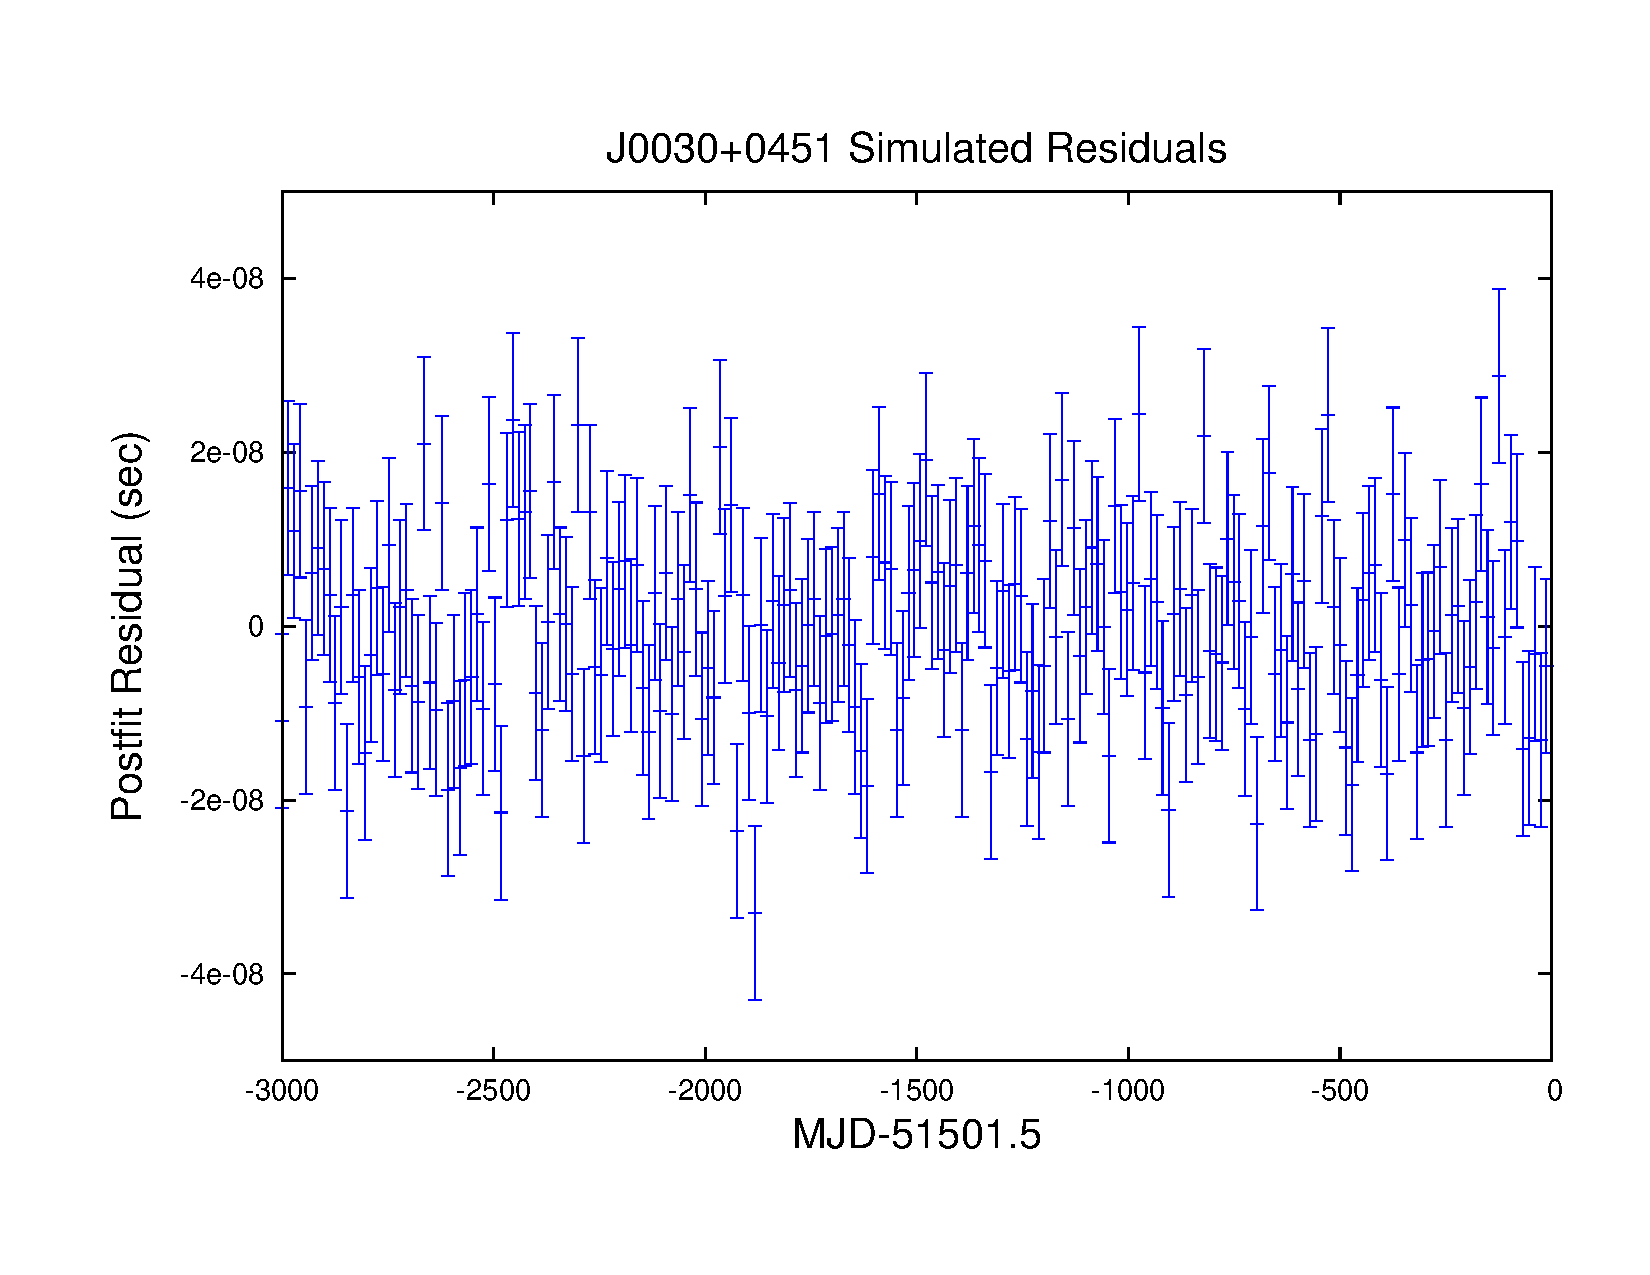
\includegraphics[width=160mm]{Sim1.pdf} \\
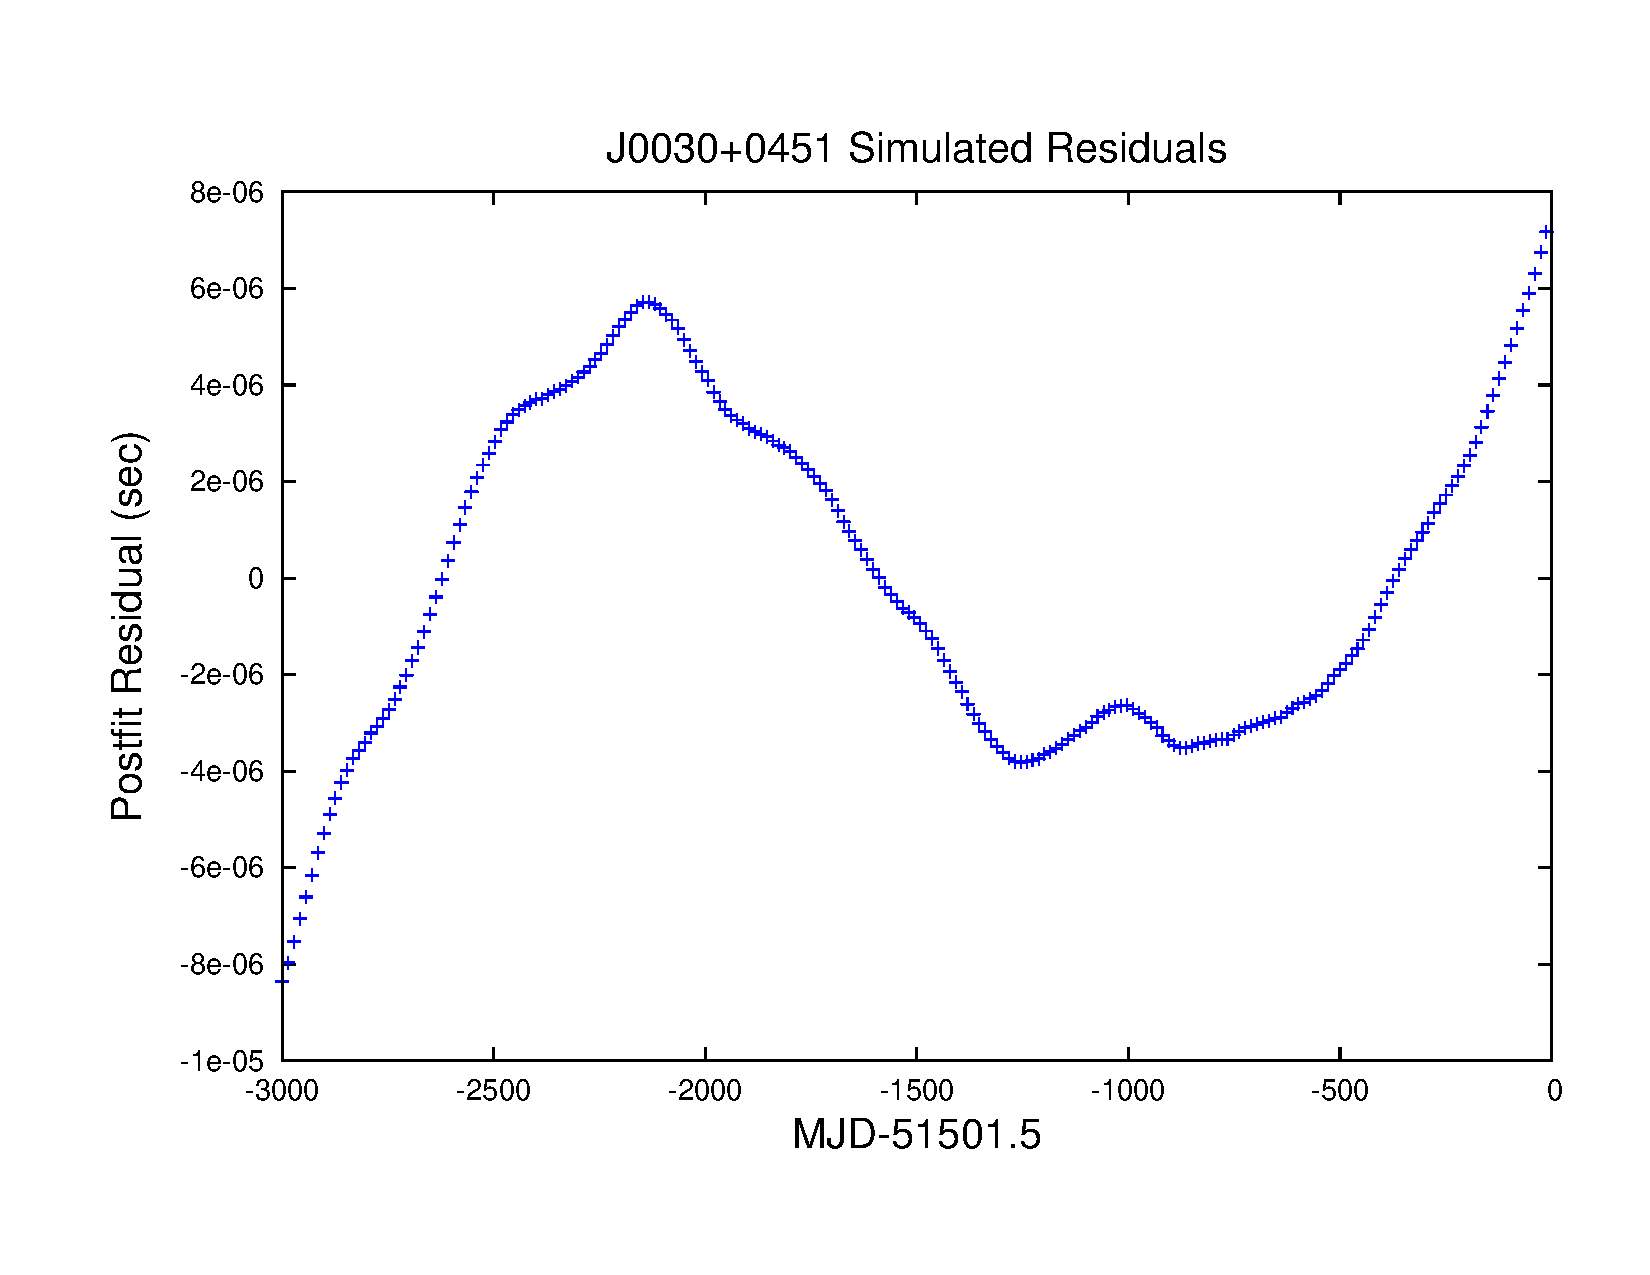
\includegraphics[width=160mm]{Sim2.pdf} \\
\end{array}$
\end{center}
\caption{}
\label{Fig:SimFigs}
\end{minipage}
\end{figure*}




\section{Output}
\label{Section:Output}


The output of TempoNest can be divided into two categories, those files that are produced by MultiNest directly, and those that are produced by TempoNest after the analysis is complete.  The former are described in the MultiNest README file, however for completion we will include the description below, followed by a summary of the TempoNest output.

\subsection{MultiNest Output}

Progress Monitoring:

MultiNest produces a physlive.dat and ev.dat files after every 500 iterations which can be used to
monitor the progress. The format and contents of  these two files are as follows:

\begin{lstlisting}
[root]physlive.dat
\end{lstlisting}
This file contains the current set of live points. It has ndim+2 columns. The first ndim columns are the ndim
parameter values. The ndim+1 column is the log-likelihood value and
the last column is the node no. (used for clustering).

\begin{lstlisting}
[root]ev.dat
\end{lstlisting}
This file contains the set of rejected points. It has ndim+3 columns. The first ndim columns are the ndim
parameter values. The ndim+1 column is the log-likelihood value,
ndim+2 column is the log(prior mass) and the last column  is the node no. (used for clustering).

---------------------------------------------------------------------------

Posterior Files:

These files are created after every 5000 iterations of the algorithm and at the end of sampling.

MultiNest will produce five posterior sample files in the root, given by the user, as following

\begin{lstlisting}
[root].txt
\end{lstlisting}
Compatable with getdist with 2+ndim columns. Columns have sample probability, -2*loglikehood, parameter values. 
Sample probability is the sample prior mass multiplied by its likelihood and normalized by the evidence.

\begin{lstlisting}
[root]post_separate.dat
\end{lstlisting}
This file is only created if mmodal is set to T. Posterior samples for modes with local log-evidence value
greater than Ztol, separated by 2 blank lines. Format is the same as [root].txt file.

\begin{lstlisting}
[root]stats.dat
\end{lstlisting}
Contains the global log-evidence, its error and local log-evidence with error and parameter means and standard
deviations as well as the  best fit and MAP parameters of each of the mode found with local log-evidence $>$ Ztol.

\begin{lstlisting}
[root]post_equal_weights.dat
\end{lstlisting}
Contains the equally weighted posterior samples. Columns have parameter values followed by loglike value.

\begin{lstlisting}
[root]summary.txt
\end{lstlisting}
There is one line per mode with ndim*4+2 values in each line in this file. Each line has the following values 
in its column mean parameter values, standard deviations of the parameters, bestfit (maxlike) parameter values, 
MAP (maximum-a-posteriori) parameter values, local log evidence, maximum loglike value.

\subsection{TempoNest Output}

In addition to the previously mentioned files TempoNest will generate three additional files after the analysis is complete.

\begin{lstlisting}
[root]paramnames
\end{lstlisting}
Contains a list of the parameter labels for the parameters included in the model.

\begin{lstlisting}
[root]designMatrix.txt
\end{lstlisting}
This contains the elements of the design matrix for the maximum likelihood timing model parameters.  The first line contains the number of TOAs and the number of parameters in the design matrix for each TOA.  The second line lists the pulsars maximum likelihood RA and DEC in radians and the next $N_{TOA} \times N_{params}$ lines are the elements in the design matrix.

\begin{lstlisting}
[root]res.dat
\end{lstlisting}
3 columns and $N_{TOA}$ lines long.  The first column is the barycentric arrival time in MJD, the second column is the residual after subtracting the maximum likelihood timing model from the analysis, and the 3rd column is the TOA error bar in units of seconds.


\section{Examples}
\label{Section:Example}

In the following section we will provide a walk through for 3 different examples of performing an analysis with TempoNest.  The first will essentially perform the same analysis as Tempo2, with the data containing only white noise and the timing model.  The second example will then introduce red noise, and will perform the analysis using a power law red noise model whilst marginalising over the timing model at the maximum likelihood position in the joint parameter space.  Finally in the third example we will analyse a dataset that contains only eight TOAs for which Tempo2 cannot converge on a solution, setting the priors manually to explore the parameter space.  


\subsection{Example 1 : Timing Model and White Noise}


In the folder Examples/Example1 you will find two files, J0030+0451.par and J0030+0451.tim.  If you look inside the par file you will see that there are seven parameters flagged to be fit by Tempo2.  These are the source position RA and Dec, the pulsars pulse frequency and spindown F0 and F1, the pulsar's proper motion PMRA and PMDEC and  its parallax PX.  The values for these parameters listed are the values that have been injected into the simulation.

The .tim file contains the time of arrivals (TOAs) for the pulses, and the noise level, which in this example is set to $10^{-8}$ seconds for all the TOAs.  This is the correct noise level used for the simulation.

TempoNest should come configured to already run on this example, therefore the parameters in the defaultparameters.conf file are set to:

\begin{lstlisting}
numTemp2its = 1;
doLinearFit = 0;
doMax = 0;

incEFAC=0;
incEQUAD=0;
incRED=0;

FitSig=4;
\end{lstlisting}

Therefore we are setting the prior range to be $\pm 4\sigma$ of the initial fit values that Tempo2 will return, and including only the timing model in the analysis.
TempoNest can be run from the Example1 folder by:
%
\begin{lstlisting}
temop2 -gr temponest -f J0030+0451.parJ0030+0451.tim
\end{lstlisting}
%
When TempoNest first runs you will see the output from the fitting process being performed by Tempo2.   MultiNest will then begin running. When MultiNest exits you should see something similar to Table \ref{Table:Tempo2Fit}, at which point the sampling is complete, and the results should be in the output folder with names 'Example1-J0030+0451-' followed by the file type.  

TempoNest includes a simple python plotting tool to allow you to visualise the posterior probability distribution for any model parameters included in the fit.  This is located in the source directory with the other TempoNest files and is called triplot.py.  It can be used from the command line with the following syntax:

\begin{lstlisting}
python triplot.py -f Examples/Example1/results/White-J0030+0451
\end{lstlisting}
%
Which will plot a figure similar to Fig \ref{Fig:Ex1}.  This shows the one and two dimensional marginalised posterior probabilities for the parameters included in the fit, i.e. the probability that the parameter takes on a specific value.

\begin{table*}
\begin{tabular}{cccccc}
\hline\hline
\multicolumn{6}{c}{Measured Quantities for Example 1} \\ 
\hline
PARAMETER    &   Tempo2-Fit        &          TempoNest-Fit         &       Uncertainty   &Difference   &Fit\\
\hline
RAJ (rad)      &  0.132894457160795 &        0.132894457161202  &       6.0988e-11 &   4.0723e-13  &  Y \\
RAJ (hms)     &   00:30:27.4299638    &      00:30:27.4299638    &     8.3865e-07 &   5.5998e-09  & \\
DECJ (rad)   &   0.0848411931583632   &     0.0848411931571961    &    1.4192e-10 &   -1.1671e-12 &  Y \\
DECJ (dms)   &   +04:51:39.75227   &        +04:51:39.75227    &       2.9273e-05 &   -2.4073e-07 & \\
F0 ($\mathrm{s}^{-1}$)   &    205.530696088273    &      205.530696088273     &     7.4592e-15 &   0     &        Y \\
F1 ($\mathrm{s}^{-2}$)    &   -4.30603838291549e-16  &   -4.306038386639e-16  &     5.5495e-23 &   -3.7235e-25  & Y \\
PMRA (mas/yr) &   -4.05082463286022    &     -4.05078591490003    &     0.0026521 &    3.8718e-05 &  Y \\
PMDEC (mas/yr) & -5.04220311336587    &     -5.04230263648793   &      0.0061956 &    -9.9523e-05  & Y \\
PX (mas)   &     4.02332575689314   &       4.02332572975724       &   0.0015997  &   -2.7136e-08 &  Y \\
\hline
\end{tabular}
\caption{Timing model parameter estimates from TempoNest as compared to the best fit values from Tempo2.  In this example only white noise and the timing model were included, and so the parameter estimates are in excellent agreement.}
\label{Table:Tempo2Fit}
\end{table*}

\begin{figure*}
\begin{minipage}{168mm}
\begin{center}$
\begin{array}{c}
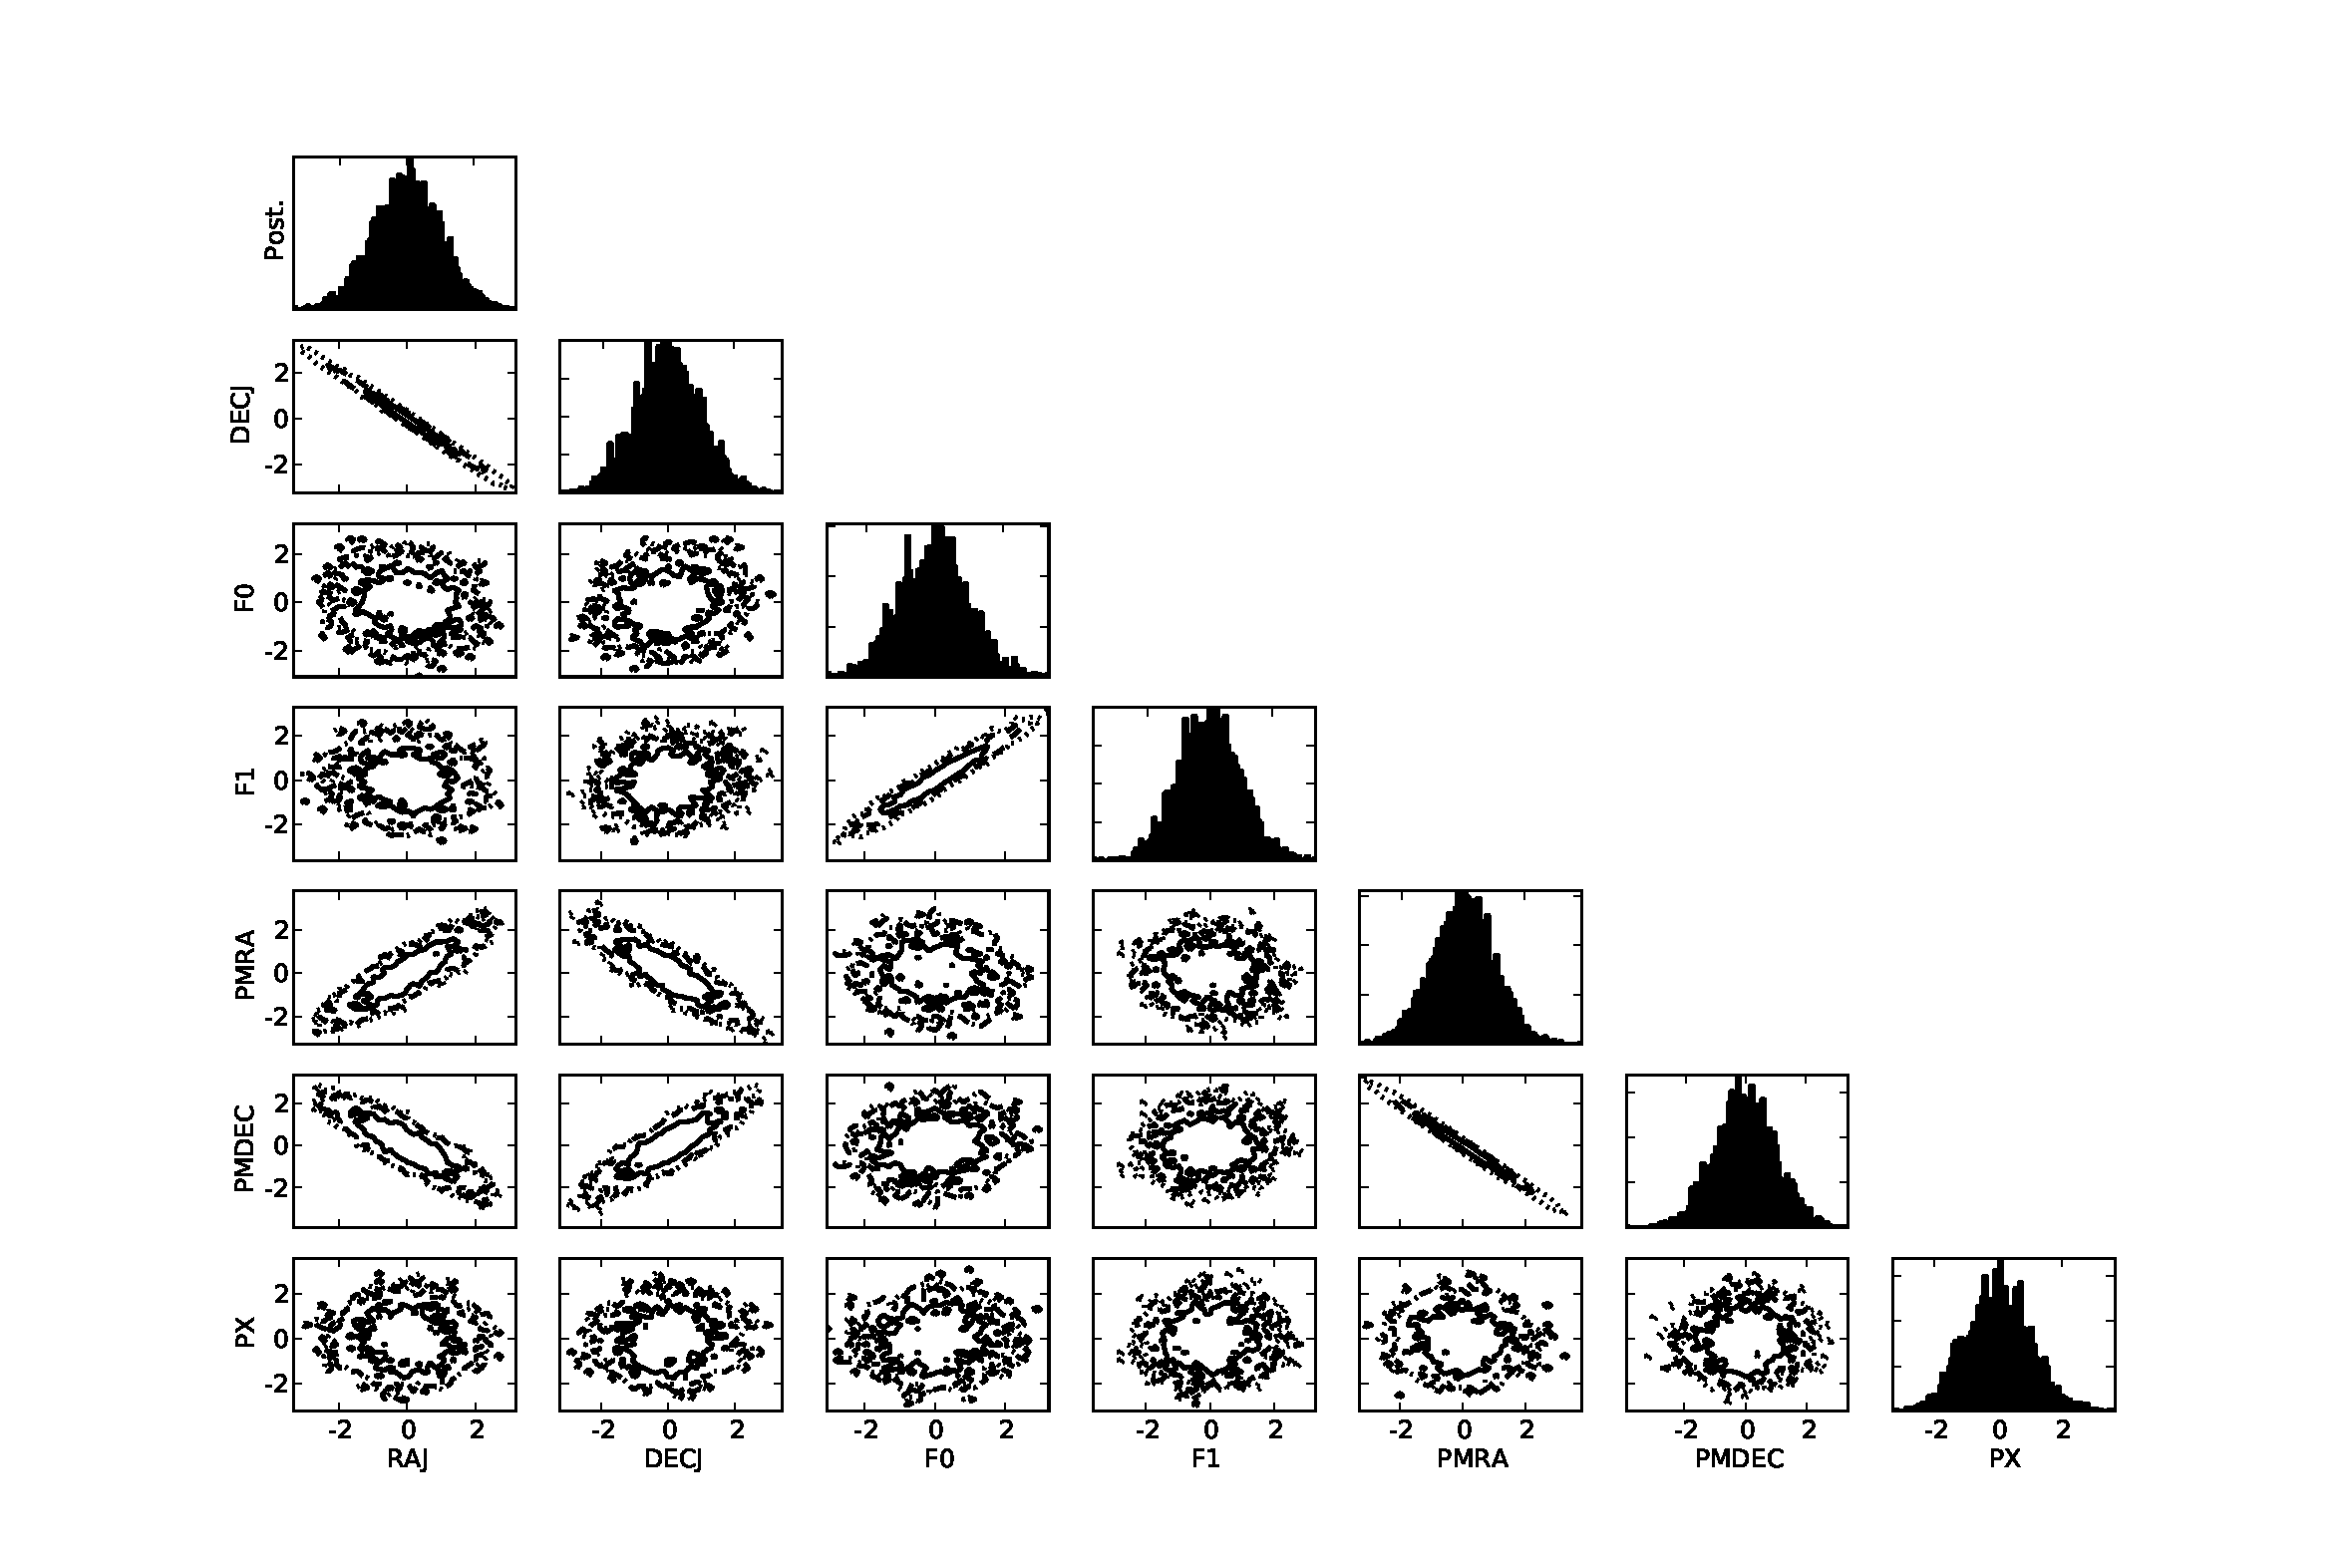
\includegraphics[width=160mm]{Example1.pdf} 
\end{array}$
\end{center}
\caption{One and two dimensional posteriors for the timing model parameters in example 1.}
\label{Fig:Ex1}
\end{minipage}
\end{figure*}


\subsection{Example 2: Timing Model and Red Noise - Power Law Model}

The tim and par files for the second example are located in Examples/Example2.  Here we have white noise and the timing model, but in addition we have added a red noise power spectrum with a log amplitude of -13.301 and spectral index of -4.333.

For the second example we will now need to change some of the parameters in the TempoNestParams.c file.  In particular we now need to change the root file name, and to specify that we wish to include a power law red noise component to out model (incRED=1).  In addition we would like to marginalise over the timing model completely (doTimeMargin=2) but would like to perform the linearisation of the timing model that is required to do this marginalisation at the maximum likelihood point for the joint parameter space (i.e. the maximum likelihood solution for the timing model when including the red noise) rather than using the initial Tempo2 fit (doMax=1). These settings are listed below.


\begin{lstlisting}
numTemp2its = 10;
doLinearFit = 0;
doMax = 1;

incEFAC=0;
incEQUAD=0;
incRED=1;

doTimeMargin=2;
doJumpMargin=0;

customPriors=0;

FitSig=10;

AlphaPrior[0] = 1.1;
AlphaPrior[1] = 6.1;

AmpPrior[0] = -15.0;
AmpPrior[1] = -12.0;
\end{lstlisting}


As before TempoNest will begin by performing the initial Tempo2 fit.  Afterwards however, instead of immediately beginning the analysis using MultiNest it will perform a maximum likelihood analysis. The final output of this should be similar to that shown below:

\begin{lstlisting}
   Max RAJ : 0.13289447885714545498 
   Max DECJ : 0.084841141721966739074 
   Max F0 : 205.5306960882738139 
   Max F1 : -4.3053954092399696773e-16 
   Max PMRA : -5.4603973577427478113 
   Max PMDEC : -1.7107901244736347262 
   Max PX : 4.1427207799322711577 
   Max Red Amp :  -13.30511142 
   Max Red Index :  3.78608546
\end{lstlisting}

TempoNest will then perform the marginalisation over the timing model parameters and perform the Bayesian analysis of the red noise spectrum the results of which should be similar to those given in Table \ref{Table:Tempo2Fit2}.

\begin{table*}
\begin{tabular}{ccc}
\hline\hline
\multicolumn{3}{c}{Measured Quantities for Example 2} \\ 
\hline
PARAMETER    &   TempoNest-Fit         &       Uncertainty  \\
\hline
Log Amplitude      &  -13.29  &        0.10   \\
Spectral Index      &   4.9  &      0.6     \\
\hline
\end{tabular}
\caption{Stochastic parameter estimates for the red noise spectrum after marginalising analytically over the timing model for Example 2.}
\label{Table:Tempo2Fit2}
\end{table*}


As before we can then plot the posterior distributions for the stochastic parameters using:


\begin{lstlisting}
python triplot.py -f Examples/Example2/results/Red-J0030+0451
\end{lstlisting}

which will display a figure similar to that in Fig \ref{Fig:Ex2}.


\begin{figure*}
\begin{minipage}{168mm}
\begin{center}$
\begin{array}{c}
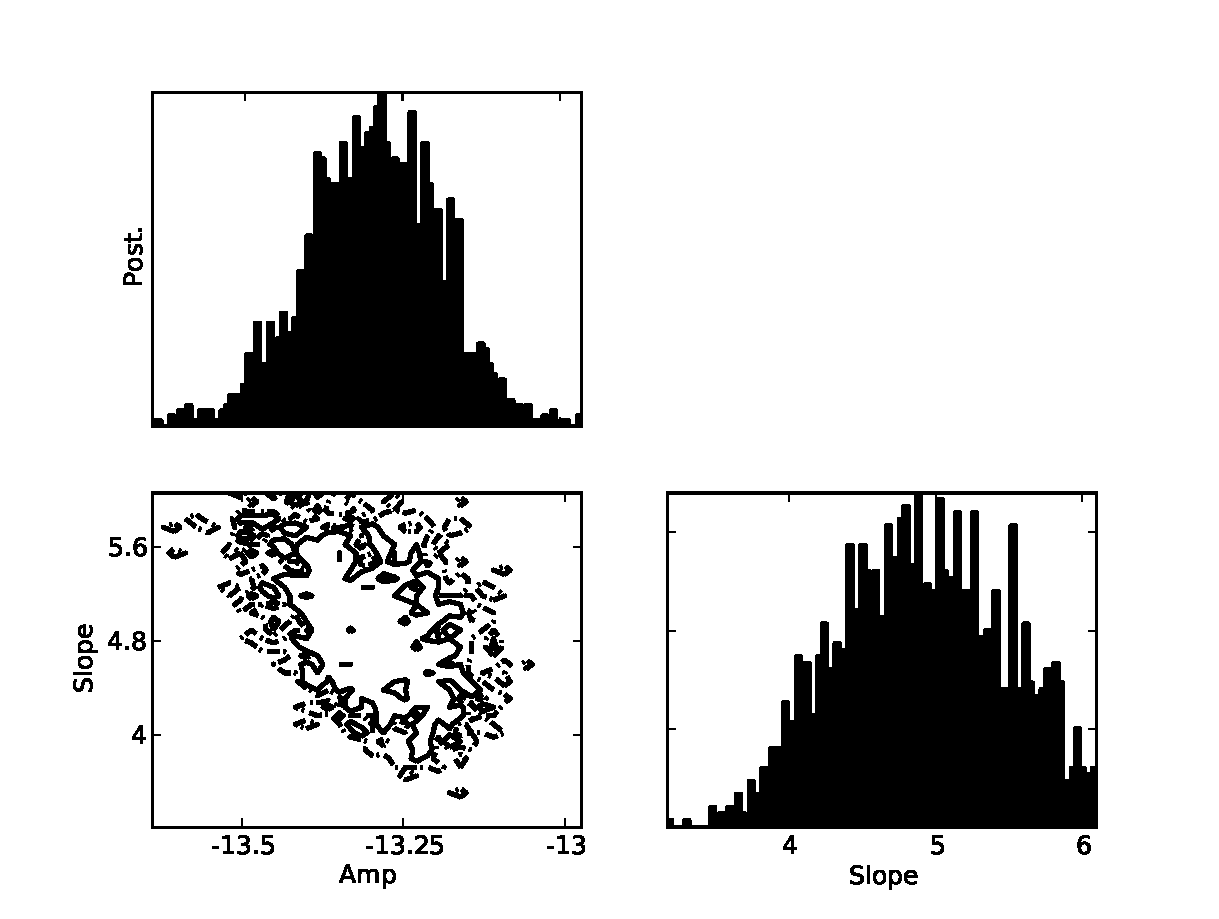
\includegraphics[width=160mm]{Example2.pdf} 
\end{array}$
\end{center}
\caption{One and two dimensional posteriors for the red noise amplitude and spectral index for example 2.}
\label{Fig:Ex2}
\end{minipage}
\end{figure*}


\subsection{Example 3: Red Noise and DM}

Example 3 contains a more complex example where both red noise and DM variations are present in the data, along with an EFAC.

Start by fitting both a red noise and DM power law model using incDM=1, incRED=1 and including an EFAC.  Compare this with incDM=3, incRED=3 for different number of fourier coefficients.  With only 10 or 20 the constraints will be worse for the latter model, but they should converge to similar values as the number of coefficients increases.  Finally try mixing the models up using incRED=3 and incDM=2 or visa versa.  The posteriors for the individual coefficients will be highly non Gaussian, and in this case the evidence will clearly support the two power law models.

This concludes the examples for TempoNest.  Feel free to generate your own data using the simulation routines and to try different models in the Bayesian analysis.  If you have any questions feel free to email me at ltl21@cam.ac.uk.



\begin{thebibliography}{}
\setlength{\labelwidth}{0pt} % fix broken mn2e.cls!

\bibitem[\protect\citeauthoryear{Feroz 
\& Hobson}{2008}]{2008MNRAS.384..449F} Feroz F., Hobson M.~P., 2008, MNRAS, 384, 449 


\bibitem[\protect\citeauthoryear{Feroz, Hobson, 
\& Bridges}{2009}]{2009MNRAS.398.1601F} Feroz F., Hobson M.~P., Bridges M., 2009, MNRAS, 398, 1601 

\bibitem[\protect\citeauthoryear{Hobbs, Edwards, 
\& Manchester}{2006}]{2006MNRAS.369..655H} Hobbs G.~B., Edwards R.~T., Manchester R.~N., 2006, MNRAS, 369, 655 

\bibitem[\protect\citeauthoryear{Hobbs, Lyne, 
\& Kramer}{2006}]{2006ChJAS...6b.169H} Hobbs G., Lyne A., Kramer M., 2006, ChJAS, 6, 020000 


\bibitem[\protect\citeauthoryear{Hobbs et al.}{2004}]{2004MNRAS.353.1311H} 
Hobbs G., Lyne A.~G., Kramer M., Martin C.~E., Jordan C., 2004, MNRAS, 353, 
1311 

\bibitem[\protect\citeauthoryear{van Haasteren 
\& Levin}{2012b}]{2012arXiv1202.5932V} van Haasteren R., Levin Y., 2012, arXiv, arXiv:1202.5932

\end{thebibliography}


\end{document}
%
% ****** End of file apstemplate.tex ******

